\chapter{Análisis complejo}
\unsection{Continuidad y limites} \label{Continuidad y limites}
Un limite en un plano complejo es muy similar a un limite en u campo vectorial. Imaginando una función $f_{(z)}=w$ que este acotada en un vecindario alrededor de $z_0$ tal que todos los puntos del intervalo estén dentro de una circunferencia de radio $\delta$ y centro $z_0$, se dice que el limite de $f_{(z)}$ en $z_0$ existe si a medida que $\delta$ sea mas pequeño $f_{(z)}$ tiende a un único valor $w$. 
\begin{figure}[H]
    \centering
    \begin{minipage}{0.49\textwidth}
    \centering
        \begin{tikzpicture}
    \draw[thin,gray!40] (0,0) grid (4,4);
    \draw[<->] (0,0)--(4,0) node[right] {$R$};
    \draw[<->] (0,0)--(0,4) node[above]{$j$};

    \coordinate (a) at (2,2);
    \coordinate (b) at (2.707,2.707);
    
    \path[fill=gray,fill opacity=0.6,dashed,line width=1pt,even odd rule] (a) circle(2) (a) circle(1);
    \draw[fill=mlgb,fill opacity=0.6,dashed,line width=1pt] (a) circle(1);
    \draw[line width=1pt,black,dashed] (a) circle(2);
    
    \draw[line width=2pt,black,-] (a) circle(1pt) node[anchor=north west]{$z_0$};
    \draw[line width=1pt,black,|-|] (a)--(b) node[midway,above,sloped]{$\delta$};
    \draw[line width=1pt,black,|-|] (a)--(0,2) node[midway,above,sloped]{$\delta_0$};
\end{tikzpicture}
\caption*{Plano $z$}
    \end{minipage}
    \begin{minipage}{0.49\textwidth}
    \centering
        \begin{tikzpicture}
    \coordinate (a) at (2,2);
    \coordinate (b) at (2.707,2.707);
    \draw[thin,gray!40] (0,0) grid (4,4);
    \draw[<->] (0,0)--(4,0) node[right] {$R$};
    \draw[<->] (0,0)--(0,4) node[above]{$j$};
    \path[fill=mlgb,fill opacity=0.6] plot[smooth cycle] coordinates {(1,1) (2,3) (3,2)};
    
    \draw[fill=gray,fill opacity=0.6,line width=1pt,dashed,even odd rule] plot[smooth cycle] coordinates {(1,0.5) (1,3) (3,3.5) (3.5,1)} plot[smooth cycle] coordinates {(1,1) (2,3) (3,2)};

    \draw[fill=black,dashed] (a) circle(2pt) node[anchor=south west] {$w_0$};
\end{tikzpicture}
\caption*{Plano $F_{(z)}$}
    \end{minipage}
    \caption{}
\end{figure}


Es importante tener en cuenta que en un plano complejo podemos acercarnos a un punto del espacio por infinitas trayectorias.


El limite se computa como en un espacio de 2 dimensiones reales. Y por lo tanto se pueden utilizar todas las herramientas del análisis real en los limites complejos.
\begin{equation}
    \begin{aligned}
         \lim_{z\to z_0} f_{(z)}=\lim_{z\to z_0} w \lrah & \lim_{z\to(x_0+jy_0)} f_{(z)}=(u_{(x,y)}+jv_{(x,y)})\\
                                         &  f_{(z_0)}=(u_{(x_0,y_0)}+jv_{(x_0,y_0)})\\
                                         &  f_{(z_0)}=w_0\\
                                         &  \lim_{z\to z_0} f_{(z)}=f_{(z_0)}=w_0
    \end{aligned}
    \label{eq:DefLim}
\end{equation}
Para que exista un función compleja se deben cumplir las mismas condiciones que en un espacio vectorial, recordándolo:
    \begin{enumerate}
        \item $\lim_{z\to z_0} f_{(z)}$ Existe
        \item $\lim_{z\to z_0} f_{(z)} = f_{(z_0)}$
    \end{enumerate}
Pero al podernos aproximar a $z_0$ por infinitas trayectorias nunca podríamos afirmar con un $100\%$ de certeza que existe un limite. Solo podríamos asegurar que no existe limite.

Un ejemplo interesante seria el de la función $z^{1/2}$ en un punto sobre el eje real negativo. Como vimos en la figura \ref{fig:z^0.5F1} esta función mapeaba todos los puntos del plano complejo $z$ sobre los cuadrantes $1$ y $4$ en el plano $w$, siendo el punto de corte el eje real negativo, entonces es razonable pensar que para un punto sobre este eje no exista limite. Planteando $\lim_{z\to z_0}$:
\begin{equation}
    \lim_{z\to z_0} f_{(z)}=\lim_{z\to z_0}z^{\frac{1}{2}}\lrah \lim_{z\to z_0} \sqrt{r}e^{j\frac{\theta}{2}}
\end{equation}
Siendo $z_0=(-1,j0)$ nos aproximándonos arbitrariamente desde 2 trayectorias circulares, la primera teniendo un argumento que se aproxima a $\pi$ del lado positivo y el segundo del lado negativo. Si nos aproximamos por el segundo cuadrante los valores de $z_0$ tenderán a $1e^{j\pi}$ y si nos aproximamos por el tercer cuadrante los valores tenderán a $1e^{-j\pi}$, planteando ambos limites:
\begin{equation}
    \begin{cases}
        \lim_{z\to z_0^{+}} \sqrt{r}e^{j\frac{\theta}{2}}=\sqrt{1}e^{j\frac{\pi}{2}}=j\\
        \lim_{z\to z_0^{-}} \sqrt{r}e^{j\frac{\theta}{2}}=\sqrt{1}e^{j\frac{-\pi}{2}}=-j
    \end{cases}
\end{equation}
Ambos limites no coinciden entonces no existe limite, como estábamos esperando.
\begin{figure}[H]
    \centering
    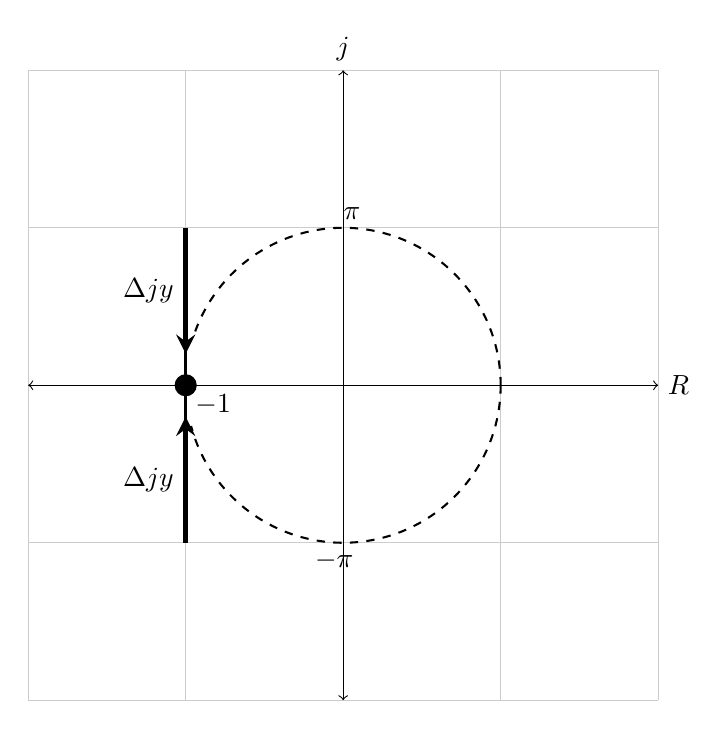
\begin{tikzpicture}[scale=2]
        \draw[thin,gray!40] (-2,-2) grid (2,2);
        \draw[<->] (-2,0)--(2,0) node[right] {$R$};
        \draw[<->] (0,-2)--(0,2) node[above]{$j$};
        \path[fill=black](-1,0) circle (2pt) node[anchor=north west]{$-1$};
        \draw[line width=0.75pt,black,dashed] (1,0) arc (0:160:1) node[midway, anchor=south east]{$\pi$};
        \draw[line width=0.75pt,black,dashed] (1,0) arc (0:-165:1) node[midway, anchor=north east]{$-\pi$};
        \draw[line width=2pt,-stealth](-1,1)--(-1,0.2) node[midway,left] {$\Delta jy$};
        \draw[line width=2pt,-stealth](-1,-1)--(-1,-0.2) node[midway,left] {$\Delta jy$};
        \draw[line width=1pt,-](-1,1)--(-1,-1);
\end{tikzpicture}
    \caption{Limite de la función $z^{1/2}$ en el punto $-1$}
    \caption{}
\end{figure}
Generalmente se puede comprobar si no existe limite en una función para cierto punto $z_0$, planteando 4 limites, 2 en dirección del eje imaginario y el otros 2 en sentido del eje real.
\begin{figure}[H]
    \centering
    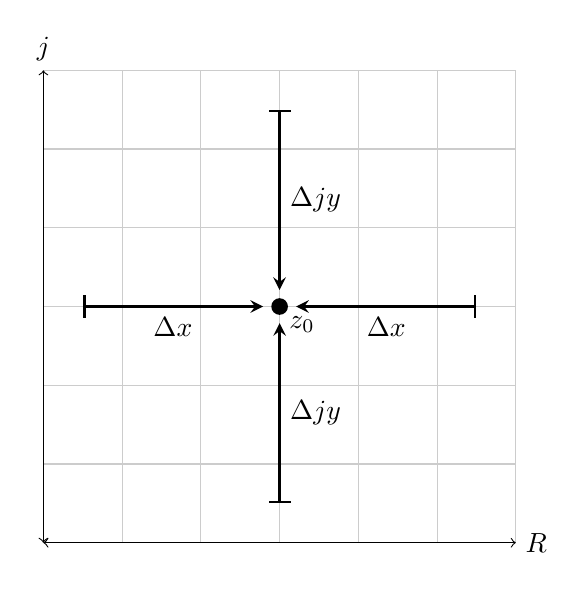
\begin{tikzpicture}
    \draw[thin,gray!40] (0,0) grid (6,6);
    \draw[<->] (0,0)--(6,0) node[right] {$R$};
    \draw[<->] (0,0)--(0,6) node[above]{$j$};

    \coordinate (a) at (3,3);
    \coordinate (b) at (2.707,2.707);
    
    \path[fill=black] (a) circle(3pt) node[anchor=north west]{$z_0$};
    \draw[line width=1pt,black,|-stealth](0.5,3)--(2.79,3) node[midway, below]{$\Delta x$};
    \draw[line width=1pt,black,|-stealth](5.5,3)--(3.21,3) node[midway, below]{$\Delta x$};
    \draw[line width=1pt,black,|-stealth](3,5.5)--(3,3.21) node[midway, right]{$\Delta jy$};
    \draw[line width=1pt,black,|-stealth](3,0.5)--(3,2.79) node[midway, right]{$\Delta jy$};
    

\end{tikzpicture}
\caption*{Plateo genérico de un limite en 4 direcciones}
    \caption{}
\end{figure}
Si en alguno de los limites planteados no da como resultado un mismo punto se puede afirmar que la función es discontinua en cierto punto $z_0$.
\unsection{Derivación y analiticidad}
La derivada en el plano complejo en un punto $z_0$ se define como:
\begin{equation}
    f'(z_0)=\lim_{\Delta z\to 0}\cfrac{f(z_0+\Delta z)-f(z_0)}{\Delta z}\lrah f'(z)=\lim_{\Delta z\to 0}\cfrac{f(z+\Delta z)-f(z)}{\Delta z}
    \label{eq:Defder}
\end{equation}
La derivada se comporta de manera similar a una función de una sola variable en su aplicación, entonces todas las derivadas inmediatas son aplicables en variable compleja. 

Para que una función sea derivable el limite debe existir independientemente de la trayectoria de $\Delta z$ como se explico en el capitulo\ref{Continuidad y limites} entonces el valor de la derivada en un mismo punto no a de cambiar según como se plante el limite. De la definición de derivada \ref{eq:Defder} y sabiendo que  $f_{(z)}=u_{(x,jy)}+jv_{(x,jy)}$ y $\Delta z=\Delta x+j\Delta y$.
\begin{equation}
    \begin{aligned}
         f'_{(z_0)}=\lim_{\Delta z\to 0}\cfrac{f(z_0+\Delta z)-f(z_0)}{\Delta z}\lrah f'_{(z_0)}=lim_{\Delta x+j\Delta y \to 0}&\cfrac{u(x_0+\Delta x,y_0+\Delta y)-u(x_0,y_0)}{\Delta x+j\Delta y}+\\
                                                                                                    &+j\cfrac{v(x_0+\Delta x,y_0+\Delta y)-v(x_0,y_0)}{\Delta x+j\Delta y}
    \end{aligned}
\end{equation}
Asumiendo que existe limite , podemos decir que aproximándonos por cualquier dirección el resultado debería ser siempre la misma derivada. Podemos identificar 2 casos de interés  uno para cuando $\Delta x=0$ aproximándonos en una dirección perpendicular al eje imaginario y otro para cuando $\Delta y=0$ aproximadnos perpendicularmente al eje real.

\begin{equation}
    \begin{cases}
        f'_{(z)}=\lim_{(\Delta x)\to 0}\cfrac{u(x+\Delta x,y)-u(x,y)}{\Delta x}+j\cfrac{v(x+\Delta x,y)-v(x,y)}{\Delta x}\\
        f'_{(z)}=\lim_{(\Delta y)\to 0}\cfrac{u(x,y+\Delta y)-u(x,y)}{j\Delta y}+j\cfrac{v(x,y+\Delta y)-v(x,y)}{j\Delta y}\\
    \end{cases}
\end{equation}
Lo que viene siendo equivalente a:
\begin{equation}
\begin{cases}
    f'_{(z)}=\cfrac{\partial u}{\partial x}+j\cfrac{\partial v}{\partial x}\\
    f'_{(z)}=\cfrac{\partial u}{j\partial y}+j\cfrac{\partial v}{j\partial y}=-j\cfrac{\partial u}{\partial y}+\cfrac{\partial v}{\partial y}
\end{cases}
\end{equation}
Agrupando e igualando las partes imaginarias y reales de este sistema obtenemos:
\begin{equation}
\begin{cases}
     \cfrac{\partial u}{\partial x}=\cfrac{\partial v}{\partial y}\\
     \cfrac{\partial u}{\partial y}=-\cfrac{\partial v}{\partial x}
     \label{eq:CauRei}
\end{cases}
\end{equation}
Por lo tanto podemos decir que cualquier función es derivable en el dominio en el cual se cumplan este sistemas de ecuaciones.
\unsubsubsection{Analiticidad}
Para que una función compleja sea analítica en un punto $z_0$, la función debe ser continua en $z_0$ y deben estar definidos dentro de la función otros infinitos puntos $z_k$ cercanos a $z_0$, derivables. Estos puntos se los suele denominar como el vecindario de $z_0$, una colección de infinitos puntos formando un disco de radio infinitesimal alrededor de $z_0$. Entones en las fronteras no definidas de una función que sea analítica una función.
\begin{figure}[H]
    \centering
    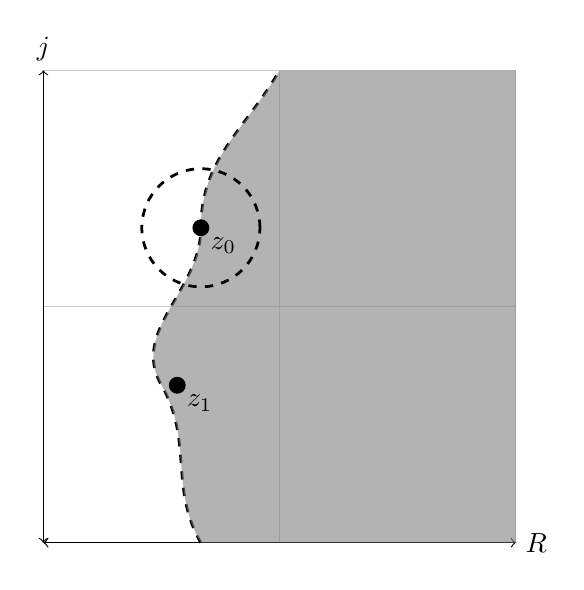
\begin{tikzpicture}
    \draw[thin,gray!40,step=3] (0,0) grid (6,6);
    \draw[<->] (0,0)--(6,0) node[right] {$R$};
    \draw[<->] (0,0)--(0,6) node[above]{$j$};

    \draw[line width=1pt,dashed,black] (2,0)to[out=120,in=-60](1.5,2)to[out=120,in=-90](2,4)to[out=90,in=-120](3,6);
    \path[fill=gray,fill opacity=0.6] (2,0)to[out=120,in=-60](1.5,2)to[out=120,in=-90](2,4)to[out=90,in=-120](3,6)--(6,6)--(6,0);
    \draw[line width=1pt,dashed,black] (2,4)circle(0.75);
    \draw[fill=black] (2,4)circle(0.1) node[anchor=north west]{$z_0$};
    \draw[fill=black] (1.7,2)circle(0.1) node[anchor=north west]{$z_1$};
    
\end{tikzpicture}
    \caption{}
    \label{fig:EjemDer}
\end{figure}
En la figura \ref{fig:EjemDer} vemos en el punto $z_0$  no existe un vecindario que no encierre algún punto fuera del dominio para el cual  la función es derivable, por lo tanto no es analítica en el punto $z_0$. En cambio para el punto $z_1$ existe un vecindario que encierre exclusivamente puntos dentro del dominio.

Las ecuaciones \ref{eq:CauRei} son las llamadas ecuaciones de \textit{Cauchy-Reiman} y tienen implicaiones muy interesantes en la integracion de funciones complejas mas adelante. Si recordamos que cualquier función $f_{(z)}$ se puede expresar como un campo vectorial expresado como:
\begin{equation}
     \begin{aligned}
         \begin{bmatrix}
           u \\
           v 
         \end{bmatrix} &= f\begin{bmatrix}
           x \\
           y 
         \end{bmatrix} 
     \end{aligned}
\end{equation}
Entonces el campo vectorial $\f{z}$ va estar dado por $(u,jv)$ los cuales están en función de $(x,y)$ del plano $z$.
Ahora si tomamos el plano $\f{z}$ y le aplicamos el operador $\nabla$ para obtener la divergencia y rotor del plano obtenemos:
\begin{equation}
    \begin{cases}
        \begin{aligned}
            \nabla & \cdot \begin{bmatrix}
                u \\
                v
            \end{bmatrix}
            =\cfrac{\partial u}{\partial x}+\cfrac{\partial v}{\partial y}
        \end{aligned}\\
        \\
        \begin{aligned}
             \nabla \times  \begin{bmatrix}
                u \\
                v
            \end{bmatrix}
            =\cfrac{\partial u}{\partial y}-\cfrac{\partial v}{\partial x}
            \end{aligned}
        \end{cases}
\end{equation}
Y si damos por echo que es un campo conservativo, es decir irrotacional y sin divergencia:
\begin{equation}
    \begin{cases}
        \begin{aligned}
            \nabla & \cdot \begin{bmatrix}
                u \\
                v
            \end{bmatrix}
            =\cfrac{\partial u}{\partial x}+\cfrac{\partial v}{\partial y}\lrah  \cfrac{\partial u}{\partial x}=-\cfrac{\partial v}{\partial y}
        \end{aligned}\\
        \\
        \begin{aligned}
             \nabla \times  \begin{bmatrix}
                u \\
                v
            \end{bmatrix}
            =\cfrac{\partial u}{\partial y}-\cfrac{\partial v}{\partial x}\lrah \cfrac{\partial u}{\partial y}=\cfrac{\partial v}{\partial x}
            \end{aligned}
        \end{cases}
\end{equation}
Estas expresiones son casi idénticas pero no iguales a las ecuaciones de \textit{Cauchy-Reiman} pero si seguimos los mismos pasos con el conjugado de $\f{z}$ (quedando $\overline{\f{z}}=(u,-v)$) vemos que la las ecuaciones de \textit{Cauchy-Reiman} están profundamente relacionadas con el roto y la divergencia del conjugado de una función:
\begin{equation}
    \begin{cases}
        \begin{aligned}
            \nabla & \cdot \begin{bmatrix}
                u \\
                -v
            \end{bmatrix}
            =\cfrac{\partial u}{\partial x}-\cfrac{\partial v}{\partial y}\lrah  \cfrac{\partial u}{\partial x}=\cfrac{\partial v}{\partial y}
        \end{aligned}\\
        \\
        \begin{aligned}
             \nabla \times  \begin{bmatrix}
                u \\
                -v
            \end{bmatrix}
            =\cfrac{\partial u}{\partial y}+\cfrac{\partial v}{\partial x}\lrah \cfrac{\partial u}{\partial y}=-\cfrac{\partial v}{\partial x}
            \end{aligned}
        \end{cases}
\end{equation}
%La relación entre el campo vectorial conjugado $\overline{\f{z}}$ y las ecuaciones de \textit{Cauchy-Reiman} se hace mas evidente en capítulos siguientes
Ahora podemos afirmar que una función es analítica en un dominio $D$ cuando en ese dominio la función conjugada es conservativa y sin divergencia. El que una función sea analítica cuando la divergencia sea igual a cero con lleva a que en el dominio en el cual se esta analizando la función no puede existir fuentes de divergencia ergo no puede existir ni "sumideros" ni "fuentes" en ese dominio. Este concepto es muy importante para la integración compleja.

\unsection{Integración}
Una función compleja, como ya sabemos, se puede expresar como un campo vectorial. Integrar en un plano complejo es entonces similar a integrar en un espacio de 2 dimensiones. Rescatando el concepto de integral de curva, integrar en un plano complejo seria la suma infinita de la multiplicación entre los vectores resultantes de una función de $z$ y infinitos segmentos infinitesimal de una curva $\gamma$ ($dz$).
\begin{equation}
    \int_\gamma f_{(z)} dz
\end{equation}
\begin{figure}[H]
    \centering
    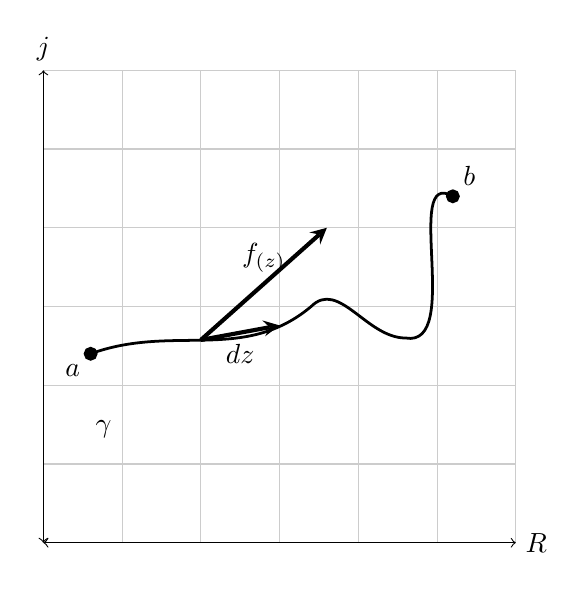
\begin{tikzpicture}[scale=2]
        \draw[step=0.5,thin,gray!40] (0,0) grid (3,3);
        \draw[<->] (0,0)--(3,0) node[right] {$R$};
        \draw[<->] (0,0)--(0,3) node[above]{$j$};
        

        \draw[line width=1pt,black] (0.3,1.2)to[out=20,in=220](1.7,1.5)to[out=45,in=180](2.3,1.3)to[out=-10,in=150](2.6,2.2);
        \draw[line width=1pt,fill=black] (0.3,1.2) circle(1pt) node[anchor=north east]{$a$};
        \draw[line width=1pt,fill=black] (2.6,2.2) circle(1pt) node[anchor=south west]{$b$};
        \draw[line width=1.5pt,-stealth] (1,1.288)--(1.8,2) node[midway, above]{$f_{(z)}$};
        \draw[line width=1.5pt,-stealth] (1,1.288)--(1.5,1.38) node[midway, below]{$dz$};
        \draw[line width=1pt] (0.5,0.6) node[anchor=south east]{$\gamma$};
         
\end{tikzpicture}
    \caption{Integral de linea sobre una curva $\gamma$}
    \label{fig:enter-label}
\end{figure}

Por ahora nos centremos en la multiplicación entre dos vectores, que es sencilla de plantear en un plano complejo.
\begin{figure}[H]
    \centering
    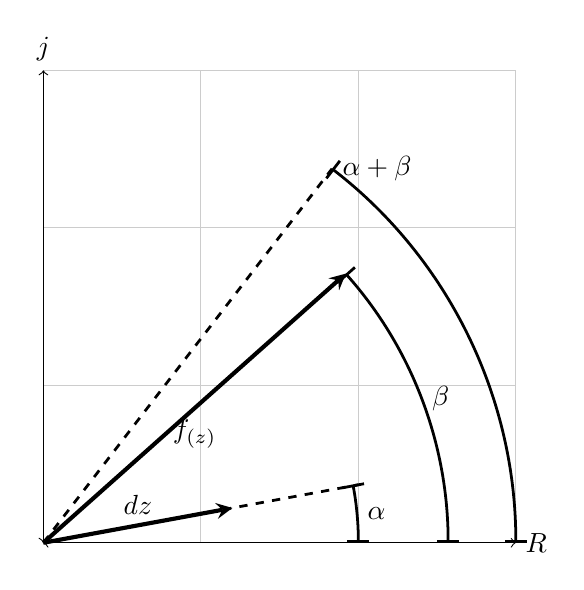
\begin{tikzpicture}[scale=2]
        \draw[thin,gray!40] (0,0) grid (3,3);
        \draw[<->] (0,0)--(3,0) node[right] {$R$};
        \draw[<->] (0,0)--(0,3) node[above]{$j$};

        \coordinate (a) at (1.6*1.2,1.424*1.2);
        \coordinate (b) at (1*2,0.184*2);
        \coordinate (c) at (1*1.2,0.184*1.2);
        \coordinate (d) at (1.833,2.375);

        \draw[line width=1.5pt,-stealth] (0,0)--(a) node[midway, below]{$f_{(z)}$};
        \draw[line width=1.5pt,-stealth] (0,0)--(c) node[midway, above]{$dz$};
        \draw[line width=1pt,dashed] (0,0)--(b);
        \draw[line width=1pt,dashed] (0,0)--(d);
        \draw[line width=1,|-|] (2.57,0) arc (0:41.67:2.57) node[midway, right]{$\beta$};
        \draw[line width=1,|-|] (2,0) arc (0:10.67:2) node[midway, right]{$\alpha$};
        \draw[line width=1,|-|] (3,0) arc (0:52.34:3) node[right]{$\alpha+\beta$};
        
\end{tikzpicture}
    
    \label{fig:enter-label}
\end{figure}
\begin{equation}
    f_{(z)} dz= |f_{(z)}||dz|e^{j(\alpha+\beta)}
\end{equation}
Podemos reescribir el argumento de la siguiente manera:
\begin{equation}
    f_{(z)} dz= |\overline{f_{(z)}}||dz|e^{j(\alpha-(-\beta))}
\end{equation}
Podemos ver que el ángulo entre el vector $dz$ y la función conjugada de $\overline{f_{(z)}}$ es igual a la suma de los argumento de la función $f_{(z)}$ y el vector $dz$.
\begin{figure}[H]
    \centering
    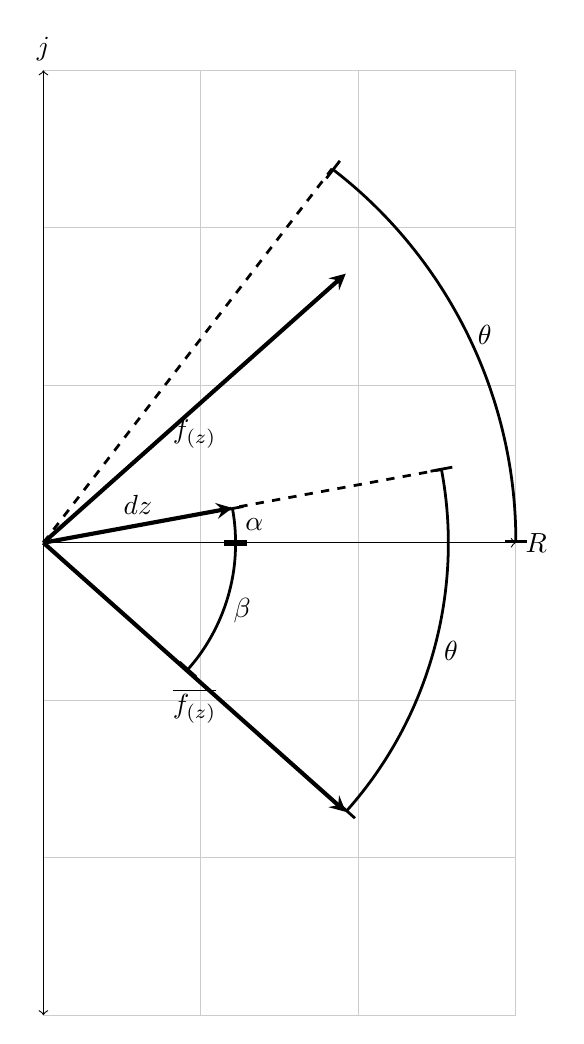
\begin{tikzpicture}[scale=2]
        \draw[thin,gray!40] (0,-3) grid (3,3);
        \draw[<->] (0,0)--(3,0) node[right] {$R$};
        \draw[<->] (0,-3)--(0,3) node[above]{$j$};
        
        \coordinate (a) at (1.6*1.2,1.424*1.2);
        \coordinate (b) at (1.6*1.2,-1.424*1.2);
        \coordinate (c) at (1*1.2,0.184*1.2);
        \coordinate (d) at (1*2.53,0.184*2.53);
        \coordinate (e) at (1.833,2.375);
        
       

        \draw[line width=1.5pt,-stealth] (0,0)--(a) node[midway, below]{$f_{(z)}$};
        \draw[line width=1.5pt,-stealth] (0,0)--(b) node[midway, below]{$\overline{f_{(z)}}$};
        \draw[line width=1.5pt,-stealth] (0,0)--(c) node[midway, above]{$dz$};
        \draw[line width=1pt,dashed] (0,0)--(d);
        \draw[line width=1pt,dashed] (0,0)--(e);
        
        \draw[line width=1,|-|] (1.22,0) arc (0:10.67:1.22) node[midway, right]{$\alpha$};
        \draw[line width=1,|-|] (1.22,0) arc (0:-41.67:1.22) node[midway, right]{$\beta$};
        \draw[line width=1,|-|] (3,0) arc (0:52.34:3) node[midway,right]{$\theta$};
        \draw[line width=1,|-|] (b) arc (-41.67:10.67:2.57) node[midway,right]{$\theta$};
        
\end{tikzpicture}
    \label{fig:enter-label}
\end{figure}
Remplazamos la exponencial compleja por la  identidad de Euler quedando:
\begin{equation}
\begin{aligned}
&\begin{aligned}
      f_{(z)} dz= |f_{(z)}||dz|e^{j(\alpha-(-\beta))} \lrah & f_{(z)} dz= |\overline{f_{(z)}}||dz|e^{j\theta} \\
                                                    & f_{(z)} dz=|\overline{f_{(z)}}||dz|(\cos{\theta}+j\sin{\theta})\\
\end{aligned}\\
&\\
 &f_{(z)} dz=|\overline{f_{(z)}}||dz|(\cos{\theta}+j\sin{\theta})
\begin{cases}
    \Real{f_{(z)} dz}=|\overline{f_{(z)}}||dz|\cos{\theta}\\
    \Imag{f_{(z)} dz}=|\overline{f_{(z)}}||dz| \sin{\theta}  
\end{cases}\\
&\\
\end{aligned}
\end{equation}
Podemos denotar que la parte real de la multiplicación entre los vectores es un producto punto. Si ahora volvemos a aplicar la integral sobre toda la expresión vemos que la parte real de esta integral es la sumatorio del producto punto entre la función y la curva $\gamma$ lo que se puede interpretar físicamente como el total de la "fuerza" aplicada a lo largo de la curva por el campo vectorial, ergo el trabajo realizado a lo largo de la curva $\gamma$.
\begin{equation}
    \int_\gamma f_{(z)}dz
    \begin{cases}
    \Real{\int_\gamma f_{(z)}dz}= \int_\gamma|\overline{f_{(z)}}||dz|\cos{\theta} \lrah \int_\gamma f_{(z)} \cdot dz \\
    \\
    \Imag{\int_\gamma f_{(z)}dz}= \int_\gamma|\overline{f_{(z)}}||dz| \sin{\theta}
    \label{eq:SubInt}
\end{cases}
\end{equation}
La parte imaginaria, sin embargo no es tan fácil de interpretar, ya que esta mas cerca de ser un producto cruz que un producto punto.

Sabiendo que $\sin{(\theta)}=\cos{(\frac{\pi}{2}-\theta)}$, podemos reinterpretar la parte imaginaria como el producto punto entre un vector normal a $dz$ de mismo modulo y el campo $\overline{f_{(z)}}$  
\begin{figure}[H]
    \centering
    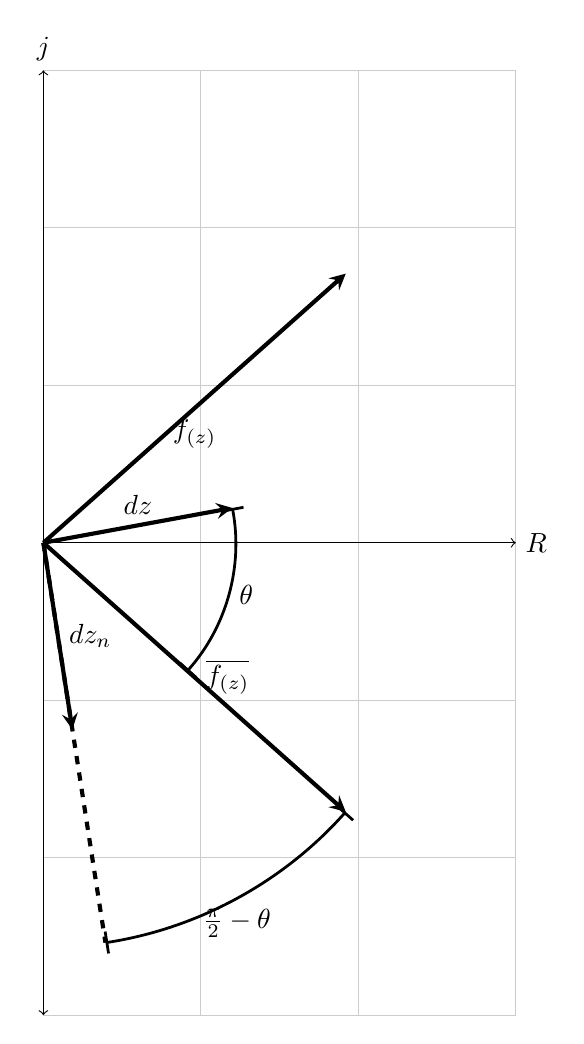
\begin{tikzpicture}[scale=2]
        \draw[thin,gray!40] (0,-3) grid (3,3);
        \draw[<->] (0,0)--(3,0) node[right] {$R$};
        \draw[<->] (0,-3)--(0,3) node[above]{$j$};
        
        \coordinate (a) at (1.6*1.2,1.424*1.2);
        \coordinate (b) at (1.6*1.2,-1.424*1.2);
        \coordinate (c) at (1*1.2,0.184*1.2);
        \coordinate (d) at (0.1533*2.57,-0.988*2.57);
        \coordinate (e) at (0.1533*1.2,-0.988*1.2);
        
       

        \draw[line width=1.5pt,-stealth] (0,0)--(a) node[midway, below]{$f_{(z)}$};
        \draw[line width=1.5pt,-stealth] (0,0)--(b) node[midway, right]{$\overline{f_{(z)}}$};
        \draw[line width=1.5pt,-stealth] (0,0)--(c) node[midway, above]{$dz$};
        \draw[line width=1.5pt,-stealth] (0,0)--(e) node[midway, right]{$dz_n$};
        \draw[line width=1.5pt,dashed] (0,0)--(d) node[midway, above]{};
        
        \draw[line width=1,|-|] (c) arc (10.67:-41.67:1.22) node[midway,right]{$\theta$};
         \draw[line width=1,|-|] (b) arc (-41.67:-81.18:2.57) node[midway,below]{$\frac{\pi}{2}-\theta$};
        
\end{tikzpicture}
    \caption{Caption}
\end{figure}
\begin{equation}
    \begin{aligned}
         |\overline{f_{(z)}}||dz| j\sin{\theta}&=j(|\overline{f_{(z)}}||dz|\cos{(\frac{\pi}{2}-\theta)}\\
                        &=j(|\overline{f_{(z)}}||dz_n|\cos{(\frac{\pi}{2}-\theta)})
    \end{aligned}
\end{equation}
La construcción de un vector $dz_n$ normal al vector $dz$ esta dado por la interpretación de un producto punto entre el vector $\overline{f_{(z)}}$ y otro vector de modulo igual a $|dz|$, que genere un ángulo de $(\frac{\pi}{2}-\theta)$ entre el mismo y $\overline{f_{(z)}}$, este ángulo siempre dará por definición un resultado que al sumarlo a $\theta$ dará $\frac{\pi}{2}$ o $90^{\circ}$ por lo tanto el vector $dz_n$ es normal a $dz$ y es de igual modulo.
Recuperando el sistema de ecuaciones \ref{eq:SubInt}:
\begin{equation}
    \int_\gamma f_{(z)}dz
    \begin{cases}
    \Real{\int_\gamma f_{(z)}dz}= \int_\gamma|\overline{f_{(z)}}||dz|\cos{\theta} \lrah \int_\gamma f_{(z)} \cdot dz \\
    \\
    \Imag{\int_\gamma f_{(z)}dz}= \int_\gamma|\overline{f_{(z)}}||-jdz|\cos{(\frac{\pi}{2}-\theta)}
\end{cases}
\end{equation}
Ahora la parte imaginaria de la integral esta asociado a un producto punto entre una normal y el vector $\overline{f_{(z)}}$. Se puede interpretar de manera física como la fuerza aplicada sobre el vector normal a $dz$ por el campo vectorial $\overline{f_{(z)}}$ o como el "flujo" del campo vectorial $\overline{f_{(z)}}$ que atraviesa el vector $dz$.

Entonces la parte imaginaria de la integral de $\f{z}$ a lo largo de una curva $\gamma$ representa el "flujo" del campo vectorial conjugado $\overline{\f{z}}$ sobre la curva $\gamma$ y la parte real el trabajo a lo largo de la curva $\gamma$.


\unsection{Series e integrales}
\unsubsection{Series}
Muchas funciones complejas son fácilmente representables a través de una serie. Representar una función en una serie es útil para entender como el teorema del residuo
